\documentclass[12pt]{amsart}
%prepared in AMSLaTeX, under LaTeX2e
\addtolength{\oddsidemargin}{-.65in} 
\addtolength{\evensidemargin}{-.65in}
\addtolength{\topmargin}{-.3in}
\addtolength{\textwidth}{1.1in}
\addtolength{\textheight}{.3in}

\renewcommand{\baselinestretch}{1.05}

\usepackage{verbatim,fancyvrb}

\usepackage{palatino}

\usepackage[dvipsnames]{xcolor}

\newtheorem*{thm}{Theorem}
\newtheorem*{defn}{Definition}
\newtheorem*{example}{Example}
\newtheorem*{problem}{Problem}
\newtheorem*{remark}{Remark}

\newcommand{\mtt}{\texttt}
\usepackage{alltt,xspace}
\newcommand{\mfile}[1]
{\medskip\begin{quote}\scriptsize \begin{alltt}\input{#1.m}\end{alltt} \normalsize\end{quote}\medskip}

\usepackage[final]{graphicx}
\newcommand{\mfigure}[1]{\includegraphics[height=2.5in,
width=3.5in]{#1.eps}}
\newcommand{\regfigure}[2]{\includegraphics[height=#2in,
keepaspectratio=true]{#1.eps}}
\newcommand{\widefigure}[3]{\includegraphics[height=#2in,
width=#3in]{#1.eps}}

\usepackage{amssymb}

\usepackage[pdftex, colorlinks=true, plainpages=false, linkcolor=black, citecolor=red, urlcolor=red]{hyperref}

% macros
\newcommand{\bb}{\mathbf{b}}
\newcommand{\bbf}{\mathbf{f}}
\newcommand{\br}{\mathbf{r}}
\newcommand{\bu}{\mathbf{u}}
\newcommand{\bv}{\mathbf{v}}
\newcommand{\bx}{\mathbf{x}}
\newcommand{\by}{\mathbf{y}}

\newcommand{\CC}{\mathbb{C}}
\newcommand{\RR}{\mathbb{R}}
\newcommand{\ZZ}{\mathbb{Z}}

\newcommand{\eps}{\epsilon}
\newcommand{\grad}{\nabla}
\newcommand{\lam}{\lambda}
\newcommand{\lap}{\triangle}

\newcommand{\ip}[2]{\ensuremath{\left<#1,#2\right>}}

%\renewcommand{\det}{\operatorname{det}}
\newcommand{\onull}{\operatorname{null}}
\newcommand{\rank}{\operatorname{rank}}
\newcommand{\range}{\operatorname{range}}

\newcommand{\Julia}{\textsc{Julia}\xspace}
\newcommand{\Matlab}{\textsc{Matlab}\xspace}
\newcommand{\Octave}{\textsc{Octave}\xspace}
\newcommand{\Python}{\textsc{Python}\xspace}

\newcommand{\prob}[1]{\bigskip\noindent\textbf{#1.}\quad }

\newcommand{\pts}[1]{(\emph{#1 pts}) }
\newcommand{\epart}[1]{\medskip\noindent\textbf{(#1)}\quad }
\newcommand{\ppart}[1]{\,\textbf{(#1)}\quad }

\newcommand*\circled[1]{\tikz[baseline=(char.base)]{
            \node[shape=ellipse,draw,inner sep=2pt] (char) {#1};}}


\begin{document}
\scriptsize \noindent Math 426 Numerical Analysis (Bueler) \hfill 20 November 2024
\normalsize

\medskip\bigskip

\Large\centerline{\textbf{Assignment \#9}}
\large
\bigskip

\centerline{\textbf{Due Monday, 2 December 2024, at the start of class}}
\medskip
\normalsize

\thispagestyle{empty}

\begin{quote}
{\small
This Assignment is based on Chapter 11 of our textbook.\footnote{Greenbaum \& Chartier, \emph{Numerical Methods: Design, Analysis, and Computer Implementation of Algorithms}, Princeton University Press 2012).}  Please read all of sections 11.1 and 11.2; the latter is very substantial!  You can skip section 11.3, but please read section 11.4 through page 289; you can skip the rest (pages 290--294).

\medskip
\noindent These expectations always apply to homework:
\renewcommand{\labelenumi}{\arabic{enumi}.\,}
\begin{enumerate}
\item Please put the problems in the order they appear below.
\item When you use \Matlab/etc, show the commands and the results.
\item Keep a clear distinction between codes, input commands, computed results, and figures.
\item Other than the text you write, please minimize use of paper.
\end{enumerate}
}
\end{quote}

\medskip
\noindent \textbf{Do these problems:}


\prob{P13}  There is a famous nonlinear ODE system which arose\footnote{It is far from obvious how this ODE system is related to the atmosphere, though the version here is now standard in textbooks.  Reading \href{https://www.tandfonline.com/doi/pdf/10.3402/tellusa.v12i3.9406}{Lorenz's original paper} is challenging, but it shows how he reduced the equations to just three.} when the programmers of the first numerical weather forecast models were trying to understand the dynamics of the atmosphere:
\begin{align*}
x'(t) &= \sigma (y - x) \\
y'(t) &= x (\rho - z) - y \\
z'(t) &= x y - \beta z
\end{align*}
Standard parameter choices for this \emph{Lorenz system} are $\sigma=10, \rho=28, \beta=8/3$.  Use \texttt{ode45()} to numerically solve this problem from initial conditions $x(0)=1$, $y(0)=1$, and $z(0)=1$, until time $T=100$.  Use \texttt{plot3()} to get a rotatable figure.  Describe in a few words what you see.

\epart{Extra Credit}  The Lorenz system exhibits a clear form of \emph{sensitive dependence on initial conditions}, in a bounded dynamical system, which is one aspect of \emph{chaos}.  By making slight changes to the initial condition, e.g.~one part in $10^8$ or less, show this sensitive dependence.  In particular, use color to distinguish two solutions which start very close in this sense, but which are on different wings of the butterfly after a not-very-long time.  To show this effect you should use tight tolerance settings for \texttt{ode45()}.

\prob{P14} \emph{This problem simplifies/clarifies Exercise 14 in Chapter 11.  Please read that Exercise for more about the physical/astronomical context.}

\medskip \noindent This problem concerns the motion of a satellite around the sun.  The satellite could be a planet, a comet, or an unpowered spacecraft.  We assume the satellite mass is small compared to the sun, and so the sun is fixed at the origin.  The coordinates of the satellite, in the plane of its orbit, are $x(t)$ and $y(t)$.  The equations for the satellite motion are Newton's laws.  In simplified units the ODE system is:
	$$x'' = \frac{-x}{(x^2+y^2)^{3/2}}, \qquad y'' = \frac{-y}{(x^2+y^2)^{3/2}}$$

\epart{a}  Re-write these two second-order ODEs into a system of 4 first-order ODEs.  Two equations in the new system define the velocities: $z(t)=x'(t)$ and $w(t)=y'(t)$.  The resulting equations can be written
    $$\bu'(t) = \bbf(\bu(t))$$
for a (column) vector $\bu(t) = [x(t), y(t), z(t), w(t)]^\top$; you are asked to precisely state the function $\bbf$.

\epart{b}  Solve the ODE system from \textbf{(a)} using Euler's method and the RK4 method.  In particular, use initial conditions $x(0)=4,y(0)=0,z(0)=0,w(0)=0.5$, and assume the duration is $T=50$.  For Euler's method use $h=0.0025$ and for RK4 use $h=0.25$.  Plot the position solution\footnote{The full solution $\bu(t)$ is in four dimensions, and not easily visualizable.} $x(t),y(t)$ for each method, and use \texttt{axis equal}.  You should see a circular orbit, with very similar results, from each method.  My code used \texttt{subplot()} to produce the Euler and RK4 results side-by-side (below).  If your code does not produce equally circular orbits then it has a bug.

\medskip
\begin{center}
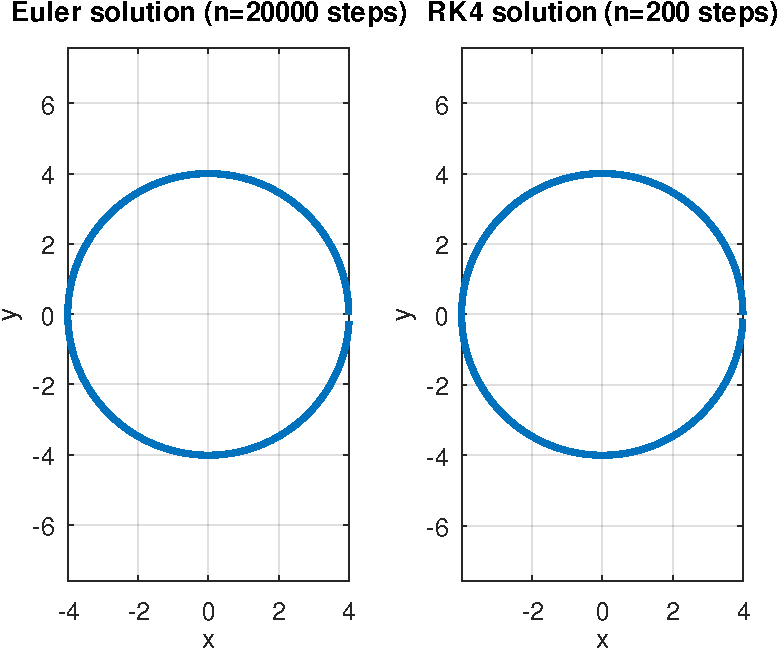
\includegraphics[width=0.5\textwidth]{figs/circleorbit.pdf}
\end{center}

\epart{c}  Fixing the other parameters, make the time step sizes $h$ substantially bigger and observe that the orbits are no longer accurate circles.  Make the steps sizes smaller and observe that you get the same circular result; results have converged at screen resolution.  Observe that Euler is terribly inefficient here.

\epart{d}  Duplicate your previous code to make a new one which only uses the RK4 method.  Repeat the experiment in \textbf{(b)}, but this time make a loop around the solver which runs these 6 cases and produces a plot for each:

\medskip
\begin{center}
\begin{tabular}{r|ccc}
case & $w(0)$ & $h$ & $T$ \\ \hline
1 & 0.5 & 0.25 & 50 \\
2 & 0.66 & 0.5 & 500 \\
3 & 0.8 & 0.5 & 200 \\
4 & 0.4 & 0.25 & 35 \\
5 & 0.2 & 0.25 & 30 \\
6 & 0.2 & 0.05 & 30
\end{tabular}
\end{center}

\medskip \noindent All other parameters have the same values as in \textbf{(b)}.  Cases 5 and 6 differ only by the step size, so they correspond to the same continuum problem, but you will see very different results.  What is going on?  Which one is closer to correct, and why?

\epart{Extra Credit}  Use \texttt{ode45()} to re-do cases 5 and 6, which will be the same because you don't specify $h$.  Adjust the relative and absolute tolerance to tighter values than the default.  Show that the adaptive time-stepping in \texttt{ode45()} is producing very short time steps when the satellite is near the sun.  Explain why this is happening, in physical terms.

\end{document}
